\documentclass[preview, 20pt]{standalone}

\usepackage{tikz}
\usetikzlibrary{shapes.geometric}
\usetikzlibrary{arrows}
\usetikzlibrary{positioning}

\tikzstyle{box} = [rectangle, minimum width=3cm, minimum height=1cm, text centered, draw=black]
\tikzstyle{arrow} = [thick,->,>=stealth]
\tikzstyle{every node}=[font=\large]

\begin{document}
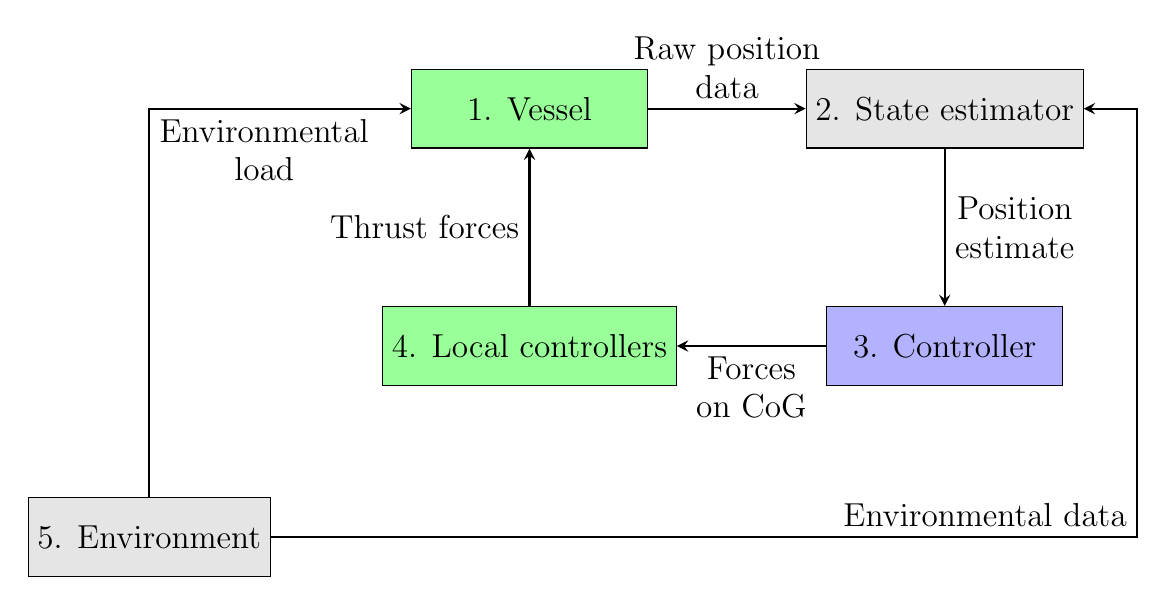
\begin{tikzpicture}[node distance = 2cm]

\node (vessel) [box, fill = green!40]{1. Vessel};
\node (state) [box, right= of vessel, fill=black!10]{2. State estimator};
\node (controller) [box, below= of state , fill=blue!30]{3. Controller};
\node (local) [box, below=of vessel, fill=green!40]{4. Local controllers};
\node (environment) [box, below left= of local, fill=black!10]{5. Environment};

\draw [arrow](vessel) -- node[anchor=south, align=center]{Raw position \\ data}(state);
\draw [arrow](state) -- node[anchor=west, align=center]{Position \\estimate}(controller);
\draw [arrow](controller) -- node[anchor=north, align=center]{Forces \\ on CoG}(local);
\draw [arrow](local) -- node[anchor=east, align=center]{Thrust forces}(vessel);
\draw[arrow](environment) |- node[anchor=north west, align=center]{Environmental \\load}(vessel);
\draw[arrow](environment.east) -| node[anchor=south east, align=center]{Environmental data} ++ (11,0) |- (state.east);


\end{tikzpicture}
\end{document}